\input preamble_DPO.tex
\usepackage{graphicx}

\date{3 февраля 2021}		% Дата семинара
\setcounter{s}{4}			% Номер семинара

\begin{document}


\title{Дискретная математика:\\
ориентированные графы и алгоритмы на графах}

\institute{Факультет компьютерных наук, НИУ ВШЭ}

\begin{frame}
  \titlepage
\end{frame}

\begin{frame}{Гамильтонов граф}

\defn Цикл в графе $G$ называется \acc{гамильтоновым}, если он проходит через каждую вершину $G$ ровно по одному разу.

\defn \acc{Гамильтонов граф} — граф, содержащий гамильтонов цикл.

\begin{center}
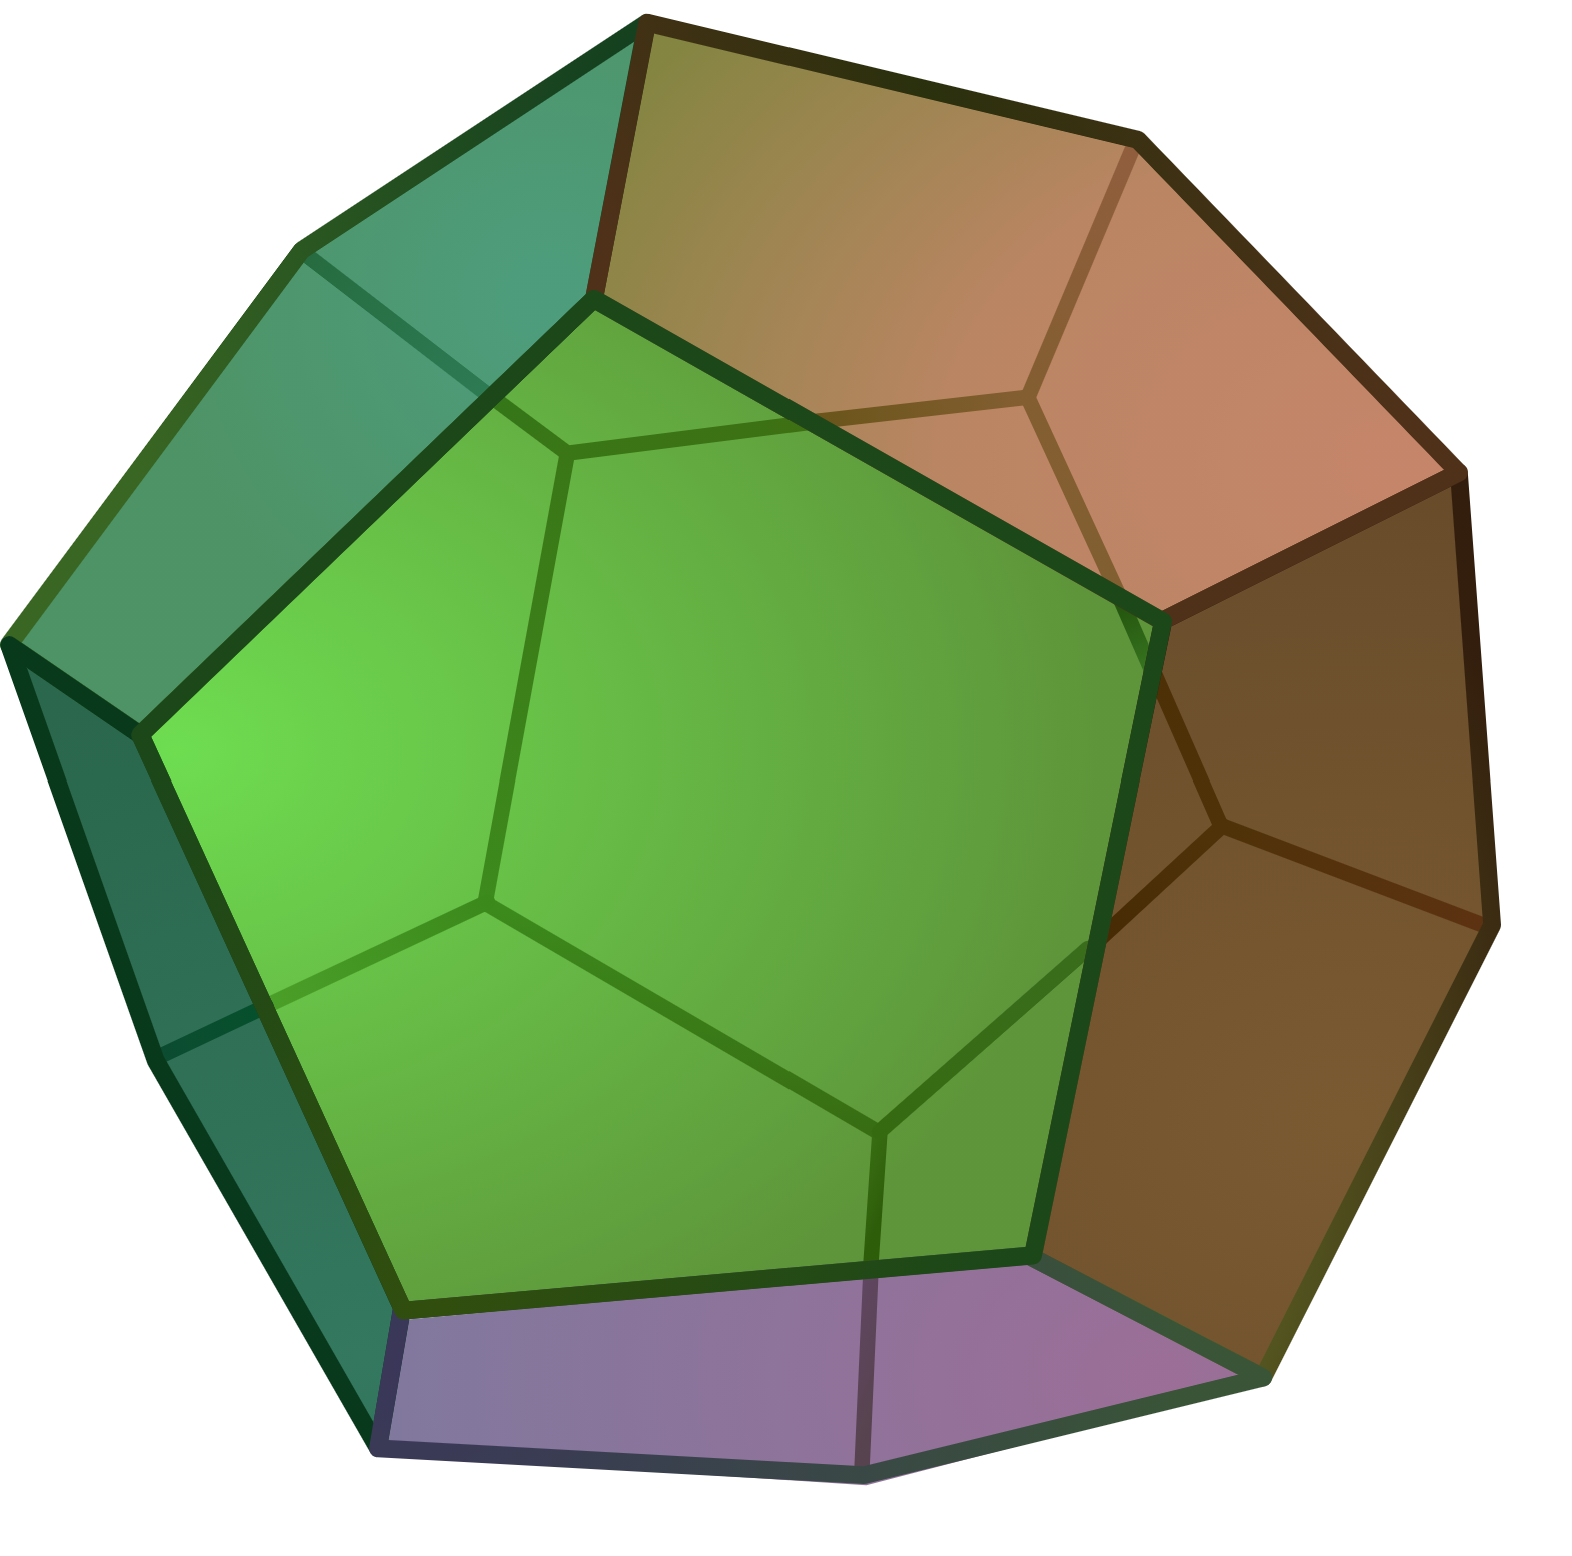
\includegraphics[scale=0.2]{img/dodecahedron.png} \textcolor{Gray}{\tiny wikipedia.org}
\end{center}



\end{frame}

\begin{frame}{Гамильтонов цикл в додекаэдре}


\begin{center}
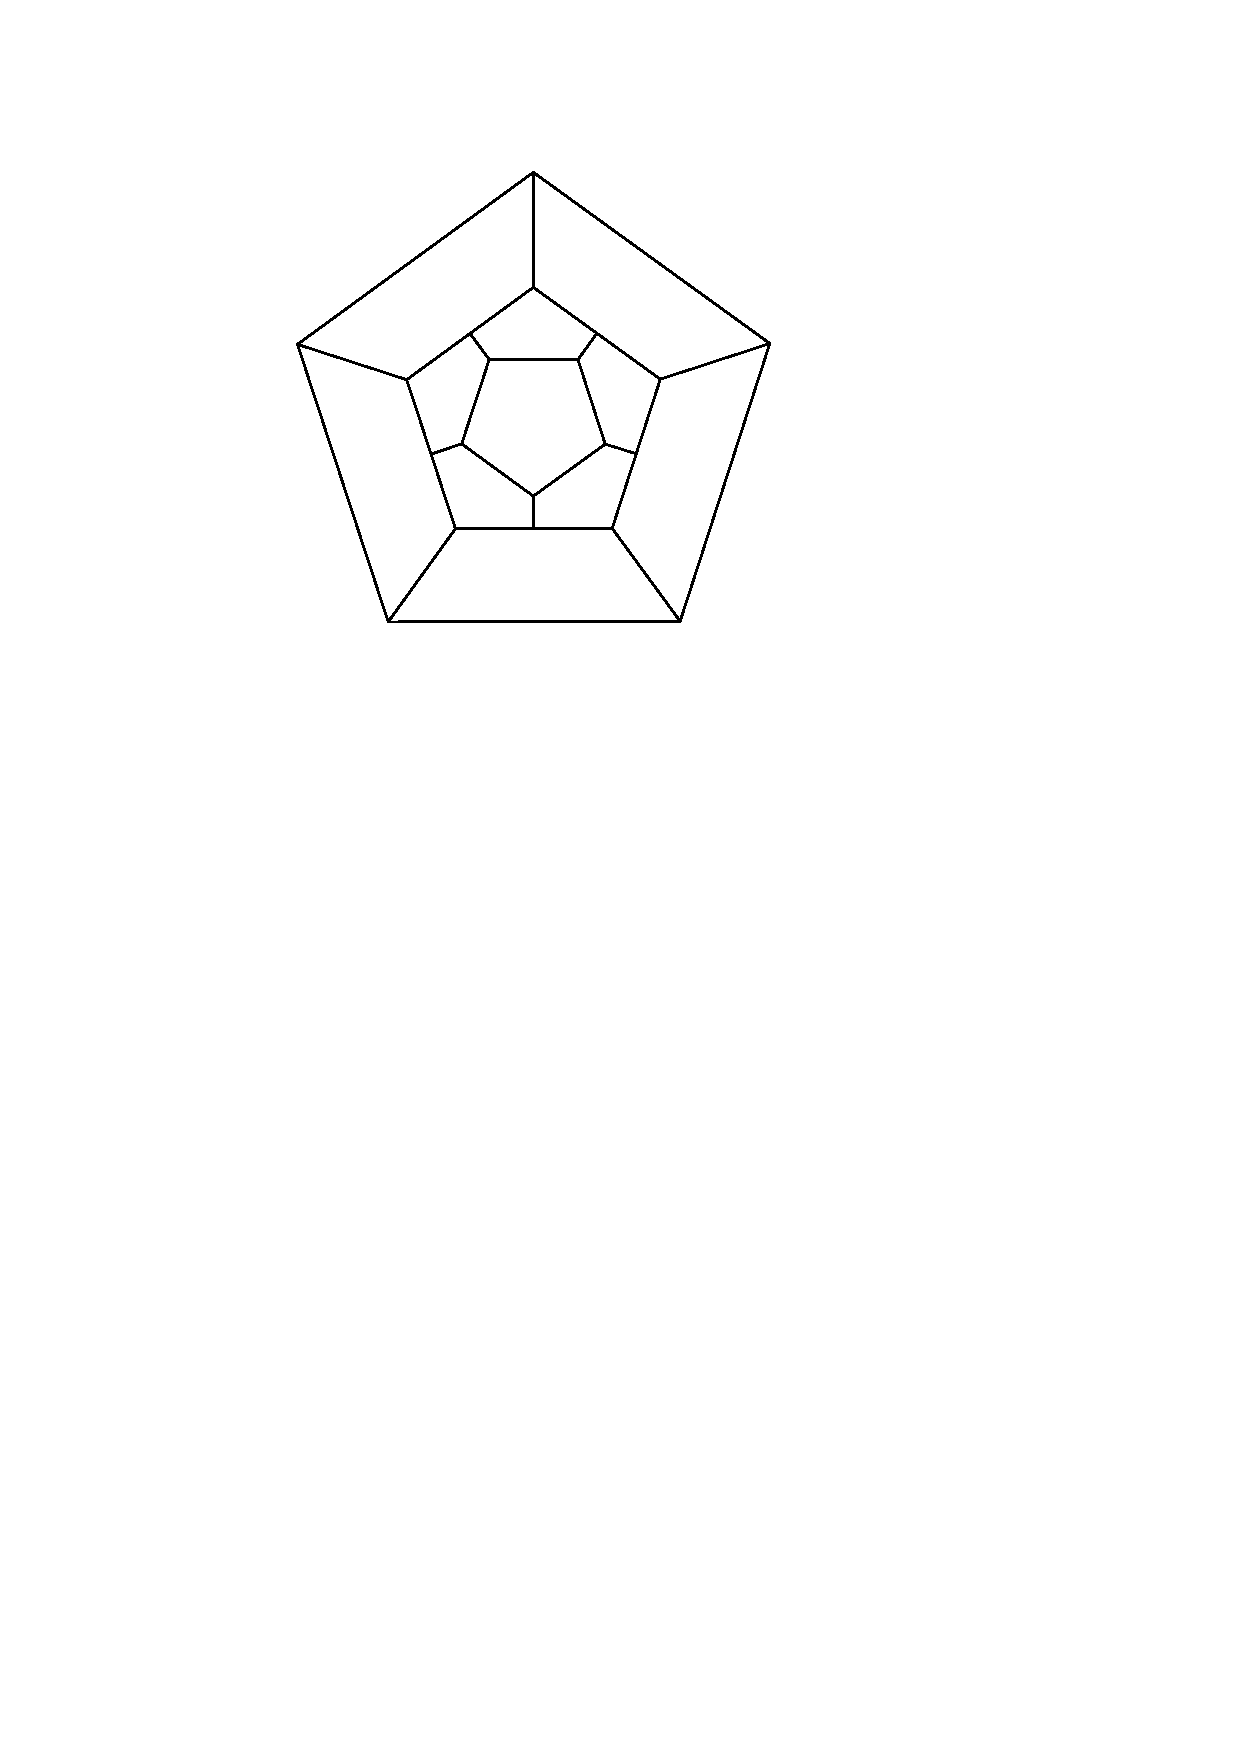
\includegraphics[scale=0.5]{img/dodecahedron.pdf} \qquad 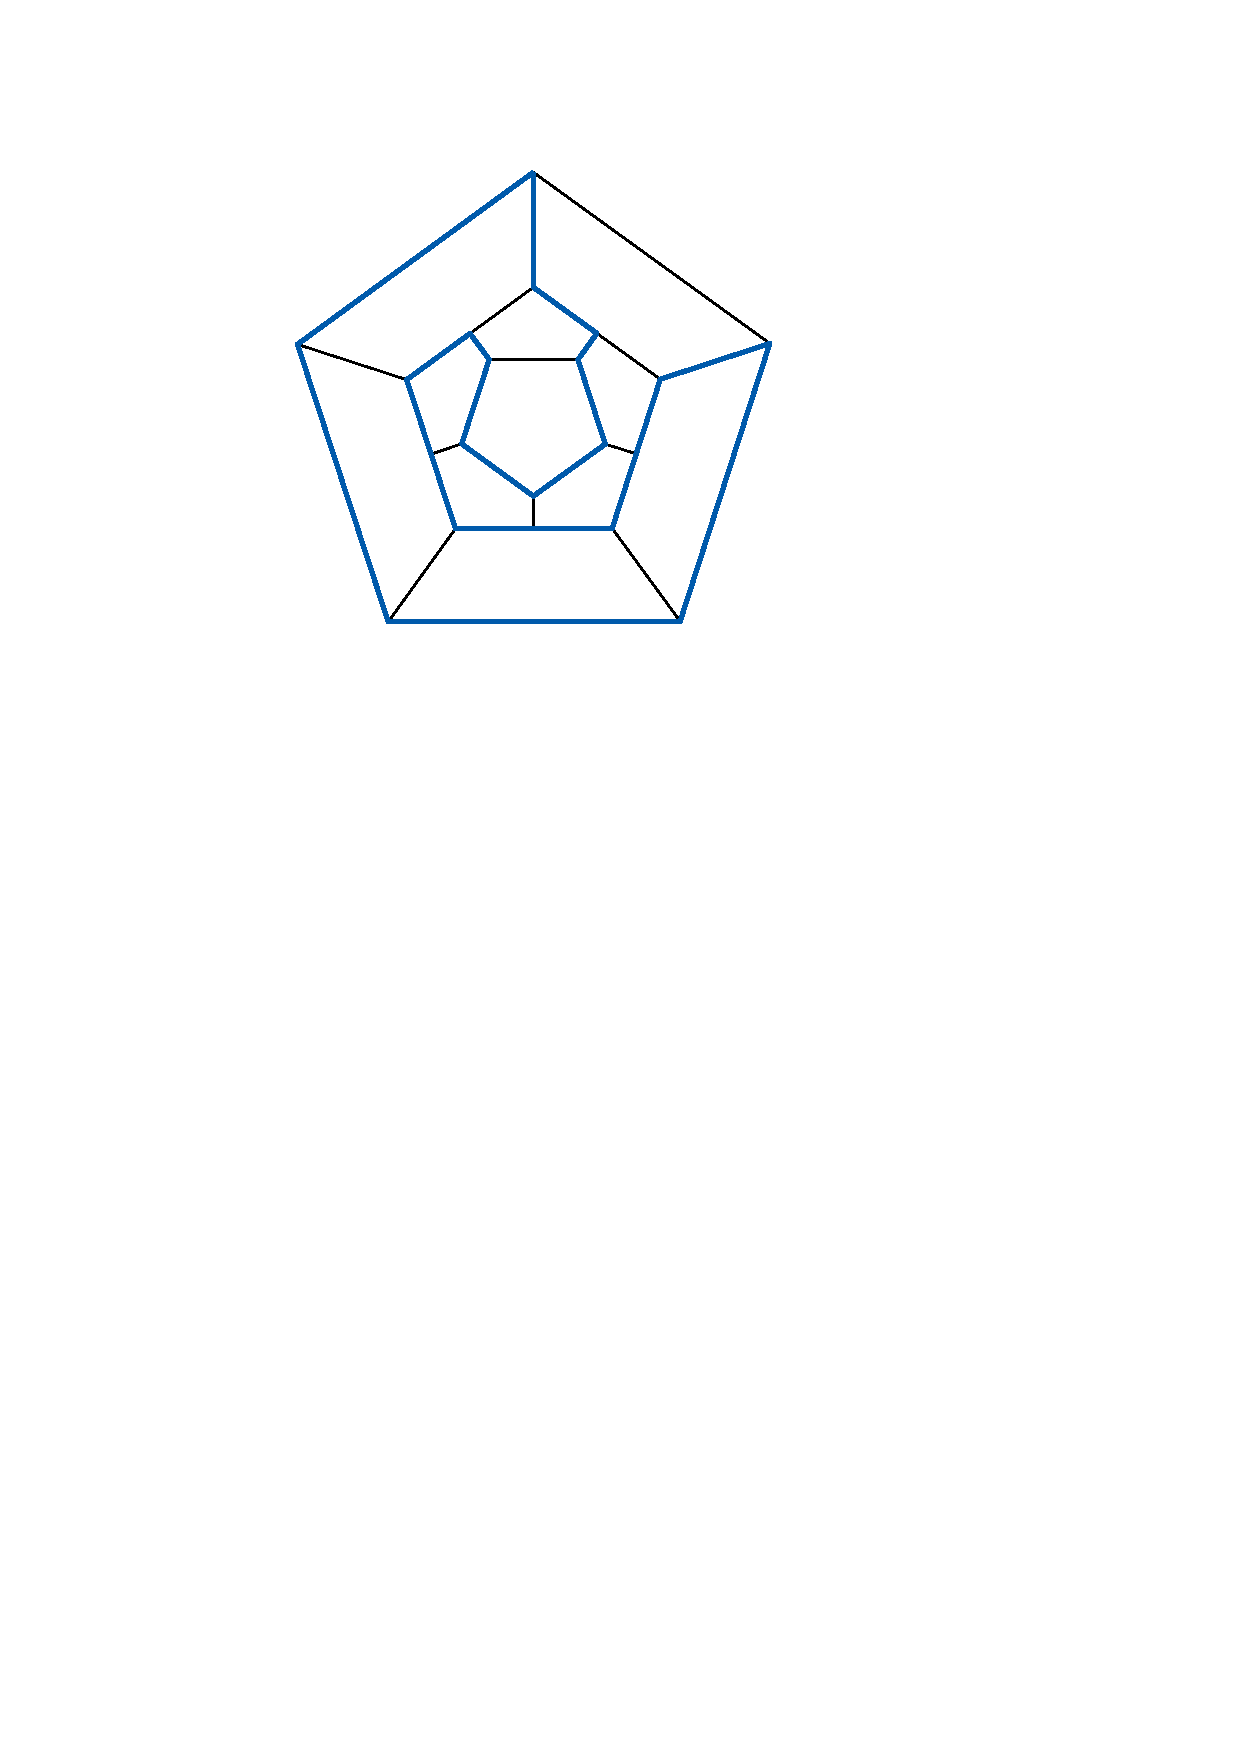
\includegraphics[scale=0.5]{img/dodecahedron2.pdf}
\end{center}

\end{frame}

\begin{frame}{Рёберный граф}

\defn Пусть задан граф $G=(V,E)$. Тогда его рёберным графом $L(G)$ называется граф с множеством вершин $E$, причем две вершины графа $L(G)$ смежны тогда и только тогда, когда соответствующие им рёбра смежны в $G$.

{\bf Теорема.} Если $G$ имеет эйлеров цикл, то $L(G)$ имеет как эйлеров, так и гамильтонов циклы.

{\bf Теорема.} Если $G$ имеет гамильтонов цикл, то $L(G)$ также имеет гамильтонов цикл.

Приложения гамильтоновых графов:

\begin{itemize}

\item \href{http://kvant.mccme.ru/pdf/2014/2014-03.pdf}{\color{blue}\underline{реконструкция генома}};

\item \href{https://en.wikipedia.org/wiki/Travelling_salesman_problem
}{\color{blue}\underline{задача коммивояжёра и транспортная логистика}}.

\end{itemize}

\end{frame}

\begin{frame}{Планарный граф}

\defn Граф называется \acc{планарным}, если его можно вложить в плоскость так, что ребра пересекаются только в вершинах графа. 

{\bf Теорема (Формула Эйлера).} Пусть в графе $G$ на $|V(G)|$ вершинах $|E(G)|$  рёбер и $|F(G)|$ граней (включая внешнюю грань). Тогда справедливо следующее соотношение:
$$|V(G)|-|E(G)|+|F(G)|=2.$$

{\bf Следствие.} $|E(G)|\leq 3|V(G)|-6.$

\exmpl Граф $K_5$ не планарный.

\exmpl {\bf(Домики и колодцы).} Граф $K_{3,3}$ не планарный.

\end{frame}

\begin{frame}{Планарный граф}

\defn Cтягивание ребра --- операция, которая удаляет ребро из графа и стягивает до этого связанные ребром вершины в одну.

\centerline{
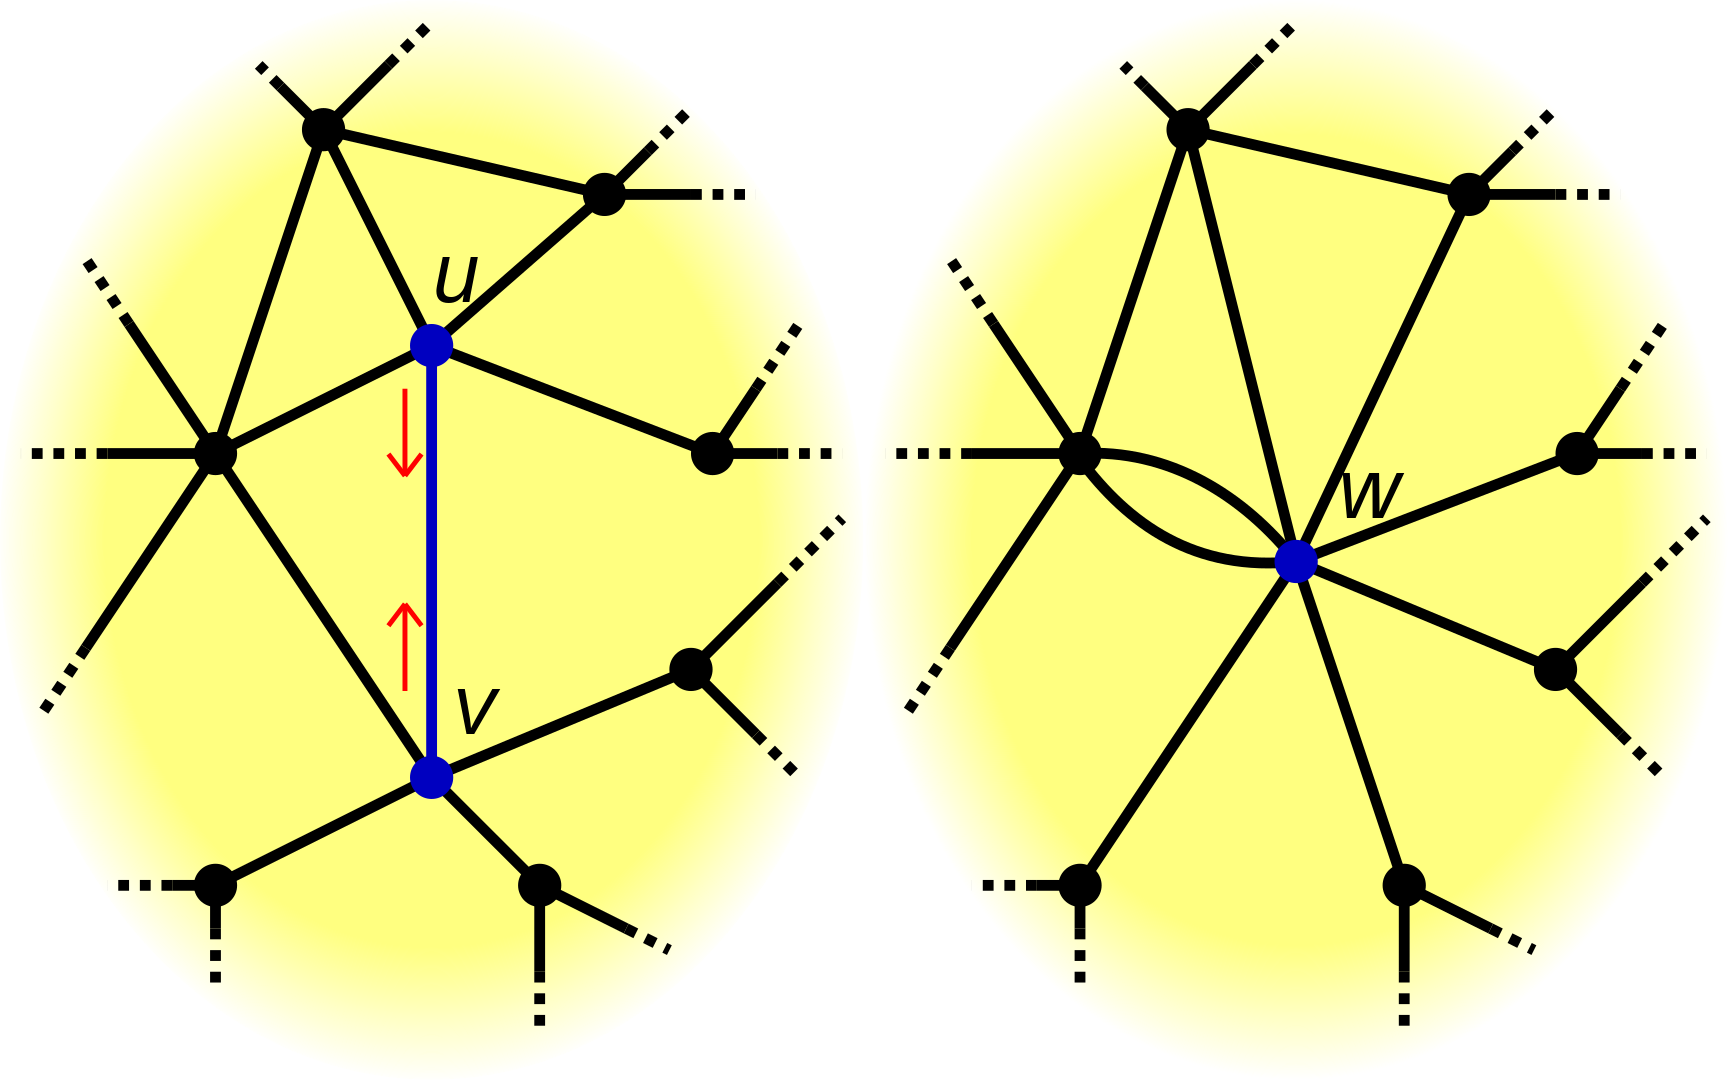
\includegraphics[width=0.4\textwidth]{img/Edge_contraction.png}

\textcolor{Gray}{\tiny wikipedia.org}
}

{\bf Теорема (Понтрягина-Куратовского).} Граф планарен тогда и только тогда, когда не содержит подграфов, стягивающихся в $K_5$ или $K_{3,3}$.

Свойства планарности очень востребованы при составлении архитектуры процессора и микросхем. Тем не менее, уже давно предпринимаются попытки по созданию \href{https://habr.com/ru/company/crossover/blog/433042/
}{\color{blue}\underline{процессора с трехмерной архитектурой}}.



\end{frame}

\begin{frame}{Ориентированные графы, мотивировка}

\exmpl В некоторой стране каждый город соединён с каждым дорогой с односторонним движением.
Докажите, что найдётся город, из которого можно добраться в любой другой.

\end{frame}


\begin{frame}{Ориентированные графы}


\defn \acc{Декартовым произведением} множеств $A$ и $B$ называют множество, состоящее из упорядоченных пар элементов из $A$ и $B$

$$A\times B=\{(a,b)\ |\ a\in A,\ b \in B\}.$$

\exmpl Множество точек на плоскости $\RR^2$, узлы решетки $\ZZ^2$, пространство $\RR^3$.

Пусть, как и раньше, $V$ --- множество вершин.

Ребра удобно рассматривать как множество пар вершин $$E\subseteq V\times V.$$

\defn Если множество ребер $E\subseteq V\times V$ состоит из упорядоченных пар, то пара $G=(V,E)$ называется \acc{ориентированным графом}.

\end{frame}


\begin{frame}{Степень в орграфе}

\defn \acc{Исходящей степенью} вершины $u$ называют число рёбер, исходящих
из $u$. Это число обозначают $\deg_{\operatorname{out}} (u)$.

\defn Аналогично определяется \acc{входящая степень} $\deg_{\operatorname{in}} (u)$ --- это число рёбер, входящих в $u$.

\exmpl Какой аналог леммы о рукопожатиях
$$\sum_{v_i\in V}\deg v_i=2|E|$$ 
справедлив для ориентированных графов?

\end{frame}


\begin{frame}{Достижимость}

\defn \acc{Ориентированный путь} --- последовательность вершин $u_1 ,u_2 ,\ldots,u_n$, в которой каждые две соседние вершины $u_i$ и $u_{i+1}$ соединены ориентированным ребром $(u_i,u_{i+1})$.

\defn Вершина $v$ \acc{достижима} из вершины $u$ в ориентированном графе, если есть ориентированный путь из $u$ в $v$.

\defn Множество состоящее из всех взаимно достижимых вершин называют \acc{компонентой сильной связности}.

\end{frame}


\begin{frame}{Сильная связность}

\begin{center}
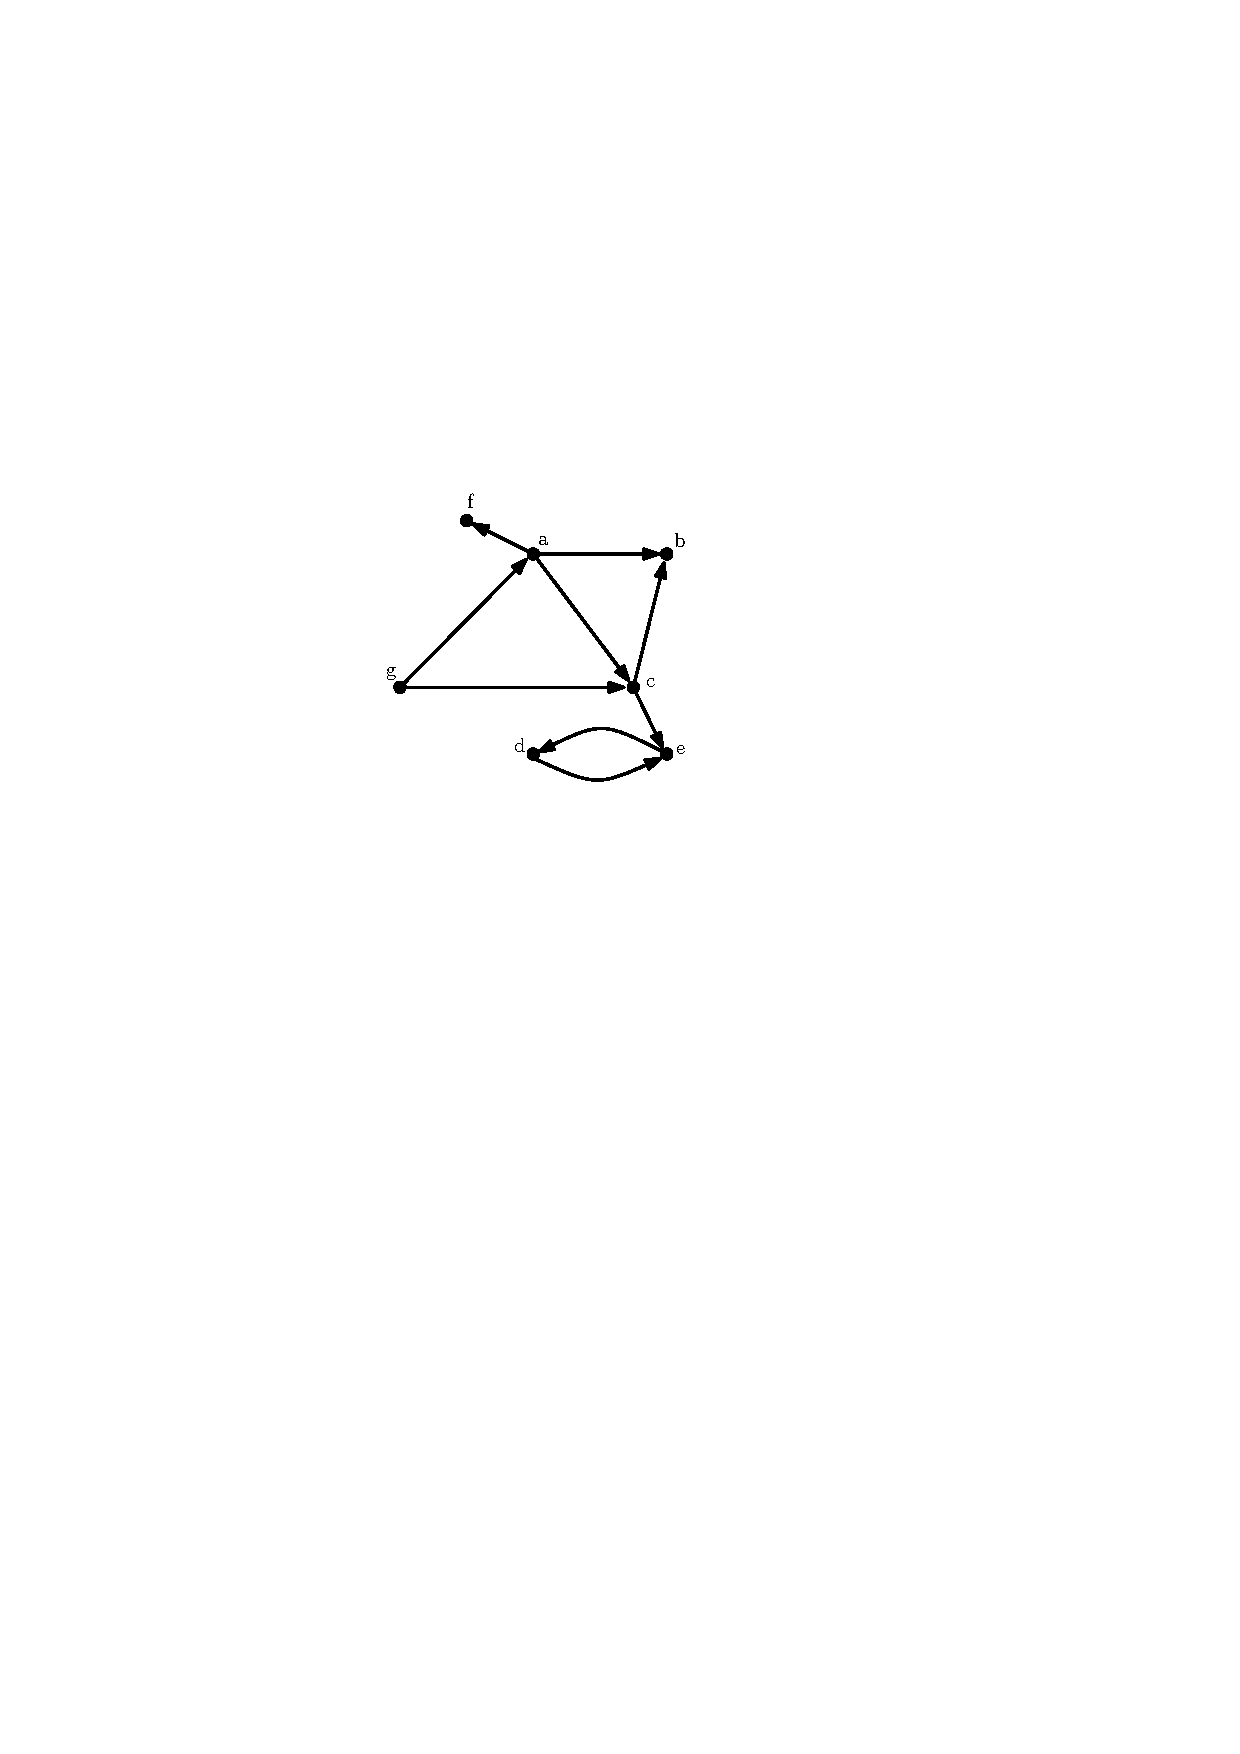
\includegraphics[scale=1]{img/digraph.pdf}
\end{center}

\exmpl Сколько компонент сильной связности содержит граф $G$?
Опишите все компоненты связности. 

\end{frame}


\begin{frame}{Алгоритм поиска в глубину}

Мы будем рассматривать алгоритм поиска в глубину как алгоритм нумерации вершин.

\begin{itemize}
\item[1.] Выбираем любую еще не занумерованную вершину $u$.
\item[2.] Запускаем процедуру $DFS(u)$:
\begin{itemize}
\item Задаем вершине $u$ минимальный еще не использованный порядковый номер.
\item Для каждой не занумерованной и смежной с $u$ вершины $v$ запускаем $DFS(v)$.
\end{itemize}

\item[3.] Повторяем шаги 1 и 2, пока все вершины не окажутся пройденными.
\end{itemize}
 
\end{frame}





\begin{frame}{Ациклические графы}

\defn Ориентированный граф называют \acc{ациклическим}, если он не содержит циклов.
\spc

Вершины ациклического графа можно рассматривать как действия, а ребра как факт того, что одно действие не может быть совершено до другого.
Поэтому ациклические графы имеют множество применений:

\begin{itemize}
\item в автоматических установщиках программного обеспечения;
\item для представления искусственных нейронных сетей без обратной связи;
\item для представления байесовской сети доверия;
\item и т.д.
\end{itemize}

\end{frame}


\begin{frame}{Ациклические графы}


\spc
{\bf Теорема.} Граф является ациклическим в точности тогда, когда вершины можно занумеровать так, что рёбра идут только от вершин с меньшим номером в вершины с большим номером.

\spc
\defn Если вершины графа занумерованы так, что рёбра идут только от вершин с меньшим номером в вершины с большим номером, то говорят, что они \acc{топологически отсортированы}.

\end{frame}

\begin{frame}{Алгоритм поиска в ширину}

А алгоритм поиска в ширину можно рассматривать и как алгоритм нумерации, и как алгоритм разбиения на уровни. 


\begin{itemize}
\item[1.] Выбираем любую еще не занумерованную вершину $u$ и задаем минимальный еще не использованный порядковый номер.
\item[2.] Запускаем процедуру $BFS(u)$:
\begin{itemize}
\item Каждому соседу вершины $u$ задаем минимальный еще не использованный порядковый номер.
\item Запускаем $BFS(v)$ для вершины $v$ с минимальным номером, у которой еще есть незанумерованные соседи.
\end{itemize}
\end{itemize}

Обход в ширину можно использовать для:
\begin{itemize}
\item нахождения расстояния между вершинами;
\item проверки на двудольность;
\item \href{https://seanperfecto.github.io/BFS-DFS-Pathfinder/}{\color{blue}\underline{нахождения выхода из лабиринта}};
\item \href{https://www.semanticscholar.org/paper/An-Algorithm-for-Path-Connections-and-Its-Lee/6b9cbd70349aac279cb69ffb6017ee6504a729b9}{\color{blue}\underline{трассировки печатных плат}};
\item и т.д.
\end{itemize}

\end{frame}


\begin{frame}{Раскраски графа}

\defn Правильной \acc{раскраской графа} называется такое сопоставление каждой его вершине цвета, что любым двум смежным вершинам соответствуют разные цвета.

\spc
{\bf Теорема о четырёх красках} --- теорема, которая утверждает, что всякую расположенную на плоскости или на сфере карту можно раскрасить не более чем четырьмя разными цветами (красками) так, чтобы любые две области с общим участком границы были раскрашены в разные цвета.

\end{frame}


\begin{frame}{Карта субъектов Российской Федерации}

\centerline{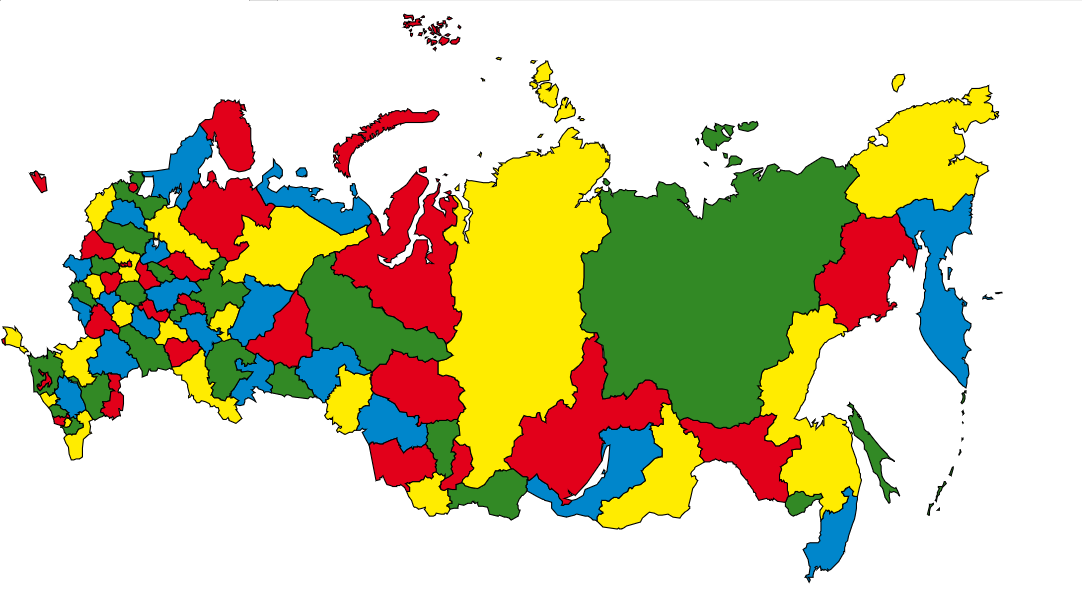
\includegraphics[scale=0.5]{img/map.png}}

\textcolor{Gray}{\tiny Автор: Insider (derivative work); Roman Poulvas (original work) - File:Map of federal subjects of Russia (2014).svg, CC BY-SA 4.0, https://commons.wikimedia.org/w/index.php?curid=51048698}

\end{frame}


\begin{frame}{Двудольные графы}

\defn Граф называется \acc{двудольным}, если его можно раскрасить в два цвета.

\exmpl В графе каждая вершина покрашена в синий или зелёный цвет. При этом каждая синяя вершина связана с пятью синими и восемью зелёными, а каждая зелёная -- с девятью синими и шестью зелёными. Каких вершин больше -- синих или зелёных?


\end{frame}


\begin{frame}{Алгоритмы раскраски}

\exmpl На территории некоторого города расположены сотовые вышки (см. рисунок). Если зоны действия вышек пересекаются, то они должны работать на разных частотах (иначе будут возникать помехи). Каждая частота стоит достаточно большую сумму денег. Сотовый оператор хочет сэкономить и использовать как можно меньше частот. Какое минимальное количество частот необходимо, чтобы покрыть весь город?


\begin{center}
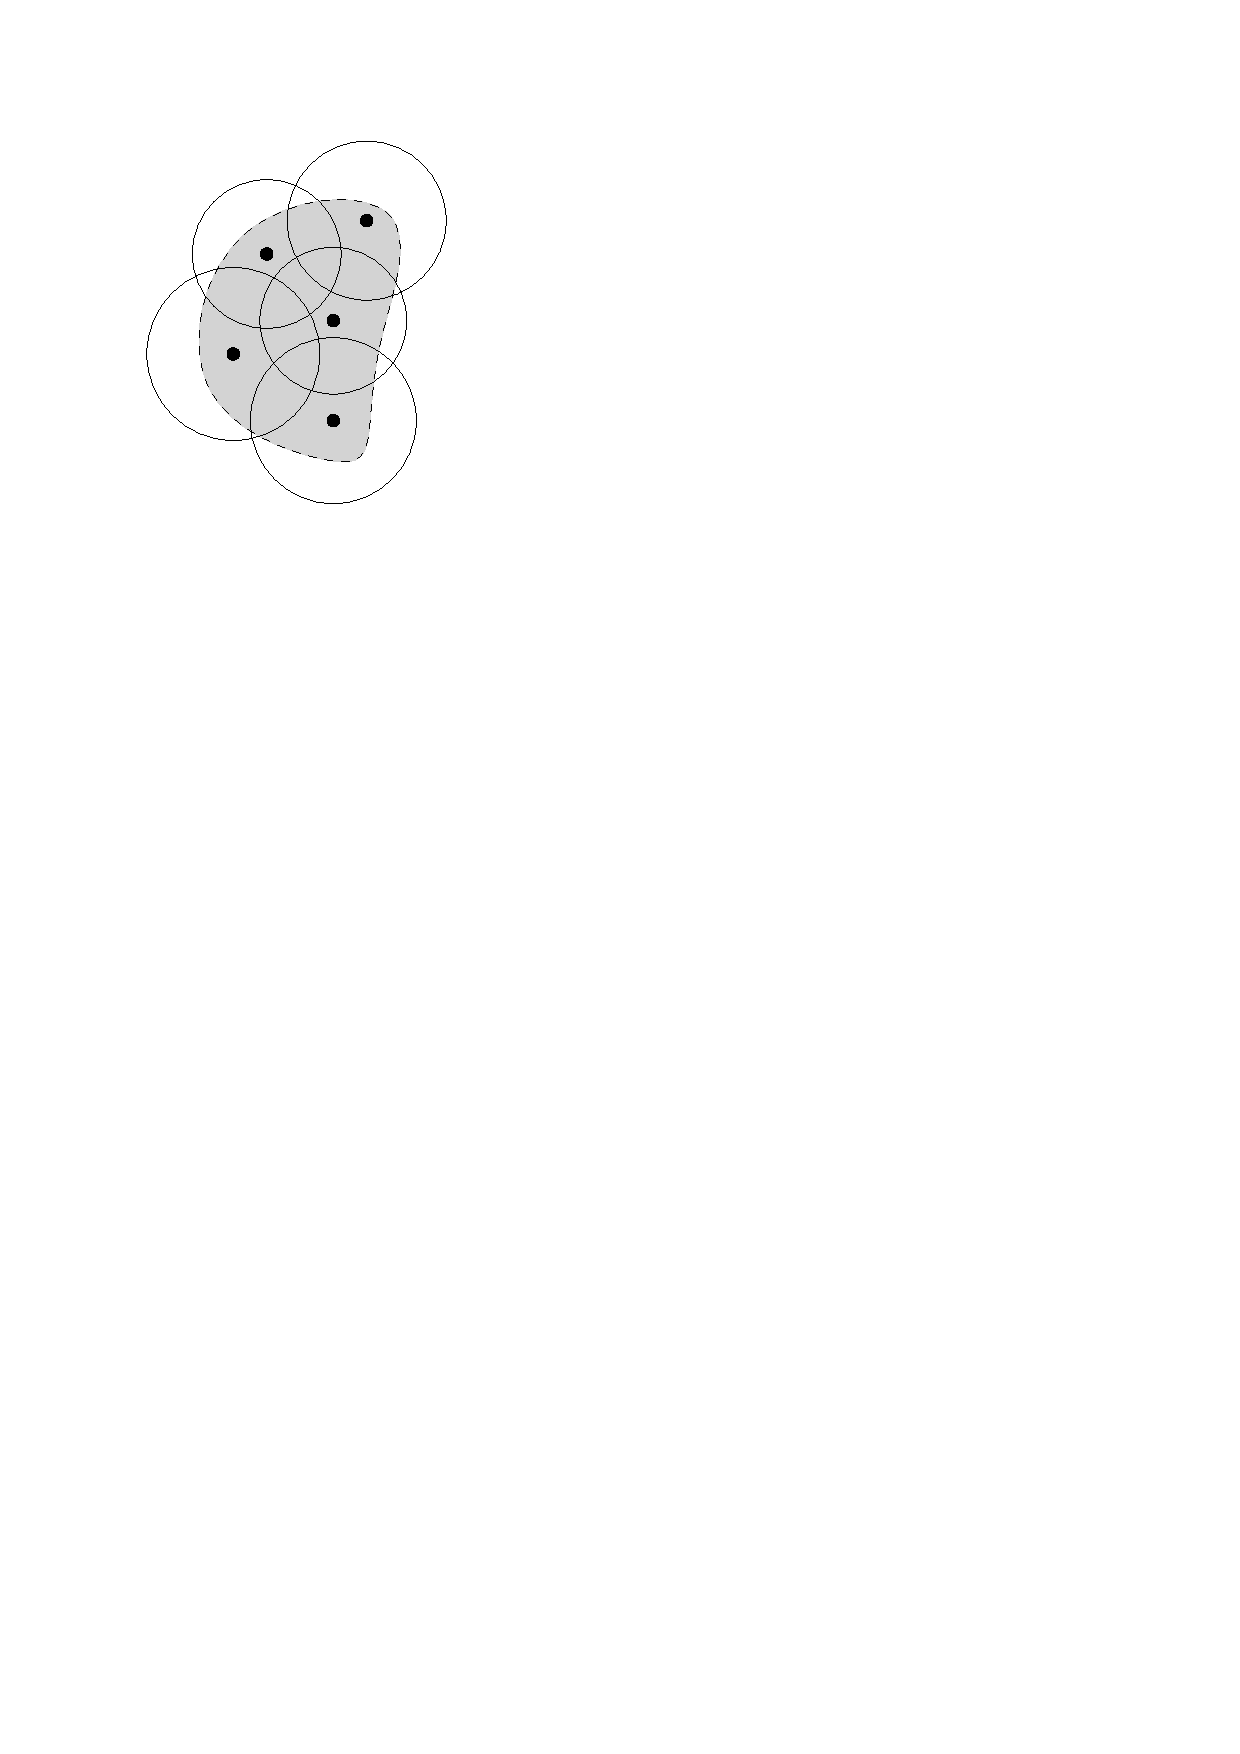
\includegraphics[scale=0.7]{img/towers.pdf}
\end{center}

\end{frame}


\begin{frame}{Немного про класс NP}{Дополнительный материал}

Информация этого слайда носит ознакомительный характер. Более подробную информацию можно найти, например, в книге

Кормен Томас Х., Лейзерсон Чарльз И., Алгоритмы. Построение и анализ. 

\defn В теории алгоритмов классом $\textbf{P}$ (от англ. polynomial) называют множество задач, для которых существуют «быстрые» алгоритмы решения (время работы которых полиномиально зависит от размера входных данных).

\defn Еще одним классом (возможно) является класс {\bf NP} (от англ. non-deterministic polynomial) множество задач с ответом <<да>> или <<нет>>, {\it решение} которых возможно проверить за полиномиальное время.

\exmpl Можно ли раскрасить граф в три цвета?

\end{frame}


\begin{frame}{Немного про класс NP}{Дополнительный материал}

Из задач класса {\bf NP} выделяют {\bf NP}-полные --- задачи, к которым можно свести любую другую задачу из этого класса за полиноминальное время.



Примеры {\bf NP}-полных задач:

\begin{itemize}
\item Задача о выполнимости булевых формул;
\item Кратчайшее решение «пятнашек» размера $n\times n$;
\item Задача коммивояжёра;
\item Проблема Штейнера;
\item Проблема раскраски графа;
\item Задача о вершинном покрытии;
\item Задача о клике;
\item Сапер (игра);
\item Тетрис;
\item и еще огромное количество задач математического программирования, теории графов и т.д.
\end{itemize}

\end{frame}


\begin{frame}{Немного про класс NP}{Дополнительный материал}

Проблема равенства классов {\bf P} и {\bf NP} является одной из семи задач тысячелетия, за решение которой Математический институт Клэя назначил премию в миллион долларов США.

\spc
Понятно, что вопрос: <<В какое минимальное число цветов можно покрасить данный граф?>> может оказаться довольно сложным.

\spc
Но это не значит, что нельзя использовать довольно оптимальные и быстрые алгоритмы решения.

\end{frame}

\begin{frame}{Жадный алгоритм раскраски}{Дополнительный материал}

\defn \acc{Жадный алгоритм раскраски:}

Пусть граф $G=(V,E)$ нужно раскрасить в цвета $c_1,c_2,c_3,\ldots$.
Упорядочим вершины $V$ произвольным образом $v_1,v_2,v_3,\ldots$. Далее последовательно раскрасим все вершины, каждый раз используя цвет с минимально возможным номером так, чтобы смежные раскрашиваемой на данном шаге вершине имели другой цвет (если они уже раскрашены).


\end{frame}

\begin{frame}{Жадный алгоритм раскраски}{Дополнительный материал}

\defn \acc{Максимальная} и \acc{минимальная} степень вершин графа $G$ обозначаются соответственно $\Delta(G)$ и $\delta(G)$.

\spc

{\bf Теорема.} Жадному алгоритму требуется не более $\Delta(G)+1$ цветов.

\end{frame}


\begin{frame}{Задачи для самостоятельного решения}

\z Докажите, что в двудольном графе сумма степеней вершин одного цвета равна сумме степеней вершин другого цвета.

\z Вершины ориентированного графа --- целые числа от $0$ до $9$. Ребро
идет из вершины x в вершину y если $y - x = 3$ или $x - y = 5$. Найдите
количество компонент сильной связности в этом графе.

\end{frame}


\begin{frame}{Задачи для самостоятельного решения}

\z Код программы содержит имена переменных $a,b,c,d,e,f,g$. При этом переменная $a$ используется в одном цикле с $b,c,e$ и $g$;
\begin{itemize}
\item значение $b$ вычисляется вместе с $d$ и $f$;

\item для вычисления $е$ требуется $g$;

\item $g$ зависит от $d$;

\item $d$ и $f$ участвуют в одной формуле.
\end{itemize}

Какое минимальное число регистров необходимо для работы программы?

\end{frame}


\begin{frame}{Задачи для самостоятельного решения}



\z Найдите наибольшее целое положительное число, в котором все цифры разные, а любые две подряд идущие цифры образуют двузначное
число, делящееся на $7$.



\z Известно, что в ориентированном графе на $n> 2$ вершинах из любой
вершины в любую другую идёт ровно один простой путь. Верно ли, что
выходные (они же исходящие) степени вершин в этом графе равны $1$?

\z В квадрате отметили $20$ точек и соединили их непересекающимися отрезками друг с другом и с вершинами квадрата так, что квадрат разбился на треугольники. Сколько получилось треугольников?

\end{frame}





\end{document}


